\part{Documento Secondo}
\chapter{Analisi dei requisiti}\label{cha:pds}
\minitoc\mtcskip
\section{Premessa}
La fase di sviluppo si strutturerà come segue:
\begin{itemize}
\diam \textit{Definizione dei diagrammi dei Casi d'Uso}

Per questa fase si mira ad effettuare una prima analisi dei casi d'uso deducibili
dal capitolato fornitoci dal cliente. In seguito all'incontro con il cliente, possiamo dedurre
i requisiti funzionali o/e comportamentali del sistema, che mostrano quali
sono i compiti base.

\diam \textit{Definizione del Testo dei Casi d'Uso}

Una volta effettuati i chiarimenti sulle specifiche con il cliente (vedi 
Sezione \vref{sec:dsicc}), si vogliono ottenere gli scenari di 
interazione con il sistema. Inoltre, per meglio venire in contro alle esigenze
dei clienti, svilupperemo queste ultime in uno \textbf{stile concreto}\footnote{C. Larman: 
Applicare UML e i Pattern. Terza edizione, edizioni Pearson Education Italia}.
Associamo inoltre i seguenti documenti:
	\begin{itemize}
	\item \textit{Glossario}:
	(v. Sezione \vref{sec:glossario}).
	\item \textit{Revisione delle stime precedenti} (v. Capitolo \vref{cha:rdsp}).
	\end{itemize}

\end{itemize}

Successivamente verranno generate, all'interno della terza fase del progetto, 
i seguenti documenti:
\begin{itemize}
\diam \textit{Definizione degli Scenari di Interazione con il sistema} %% TODO link
\diam \textit{Definizione del Modello di Progetto} %% TODO link
\end{itemize}

\section{Incontro con il cliente}\label{sec:dsicc}
\subsection{Chiarimenti sulle specifiche}\label{subsec:cssdc}
Riportiamo sotto forma di dialogo i chiarimenti sulle specifiche.

\begin{description}
\item[Q] Gli amministratori sono predefiniti, oppure bisogna crearli tramite registrazione?
\item[R] Le credenziali degli amministratori devono già essere cablate all'interno dell'applicativo, in modo da procedere unicamente con l'autenticazione. Per credenziali si intende la coppia di informazioni \textsc{Nome Utente} e \textsc{Password}: non deve essere quindi possibile la creazione di nuovi utenti amministratori.
\medskip

\item[Q] Bisogna dividere interfaccia utente da interfaccia amministratore?
\item[R] Quando si entra nell'applicazione, è possibile o accedere in modalità cliente, nella quale è possibile o effettuare un log-in, o effettuare una registrazione, oppure accedere tramite log-in o come amministratore di pediatria, o come amministratore di ortopedia.
\medskip

\item[Q] Cosa può fare un amministratore una volta autenticato?
\item[R] L'amministratore deve convalidare le richieste dei pazienti, creando la nuova prenotazione. Inoltre l'amministratore può spostare o annullare prenotazioni già convalidate, su richiesta del paziente stesso.
Ogni assegnamento di un appuntamento verrà notificato al paziente.
\medskip

\item[Q] Deve esistere un super-utente con massimo privilegio, in grado di convalidare le richieste da parte di clienti o amministratori?
\item[R] Gli unici due utenti ad avere massimo privilegio devono essere i due amministratori del reparto di pediatria e di ortopedia: non esistono altri amministratori se non questi già predefiniti. 
\medskip


\item[Q] Cosa si intende con ``maggiori permessi di manipolazione sulle prenotazioni''?
\item[R] Mentre agli utenti è permesso effettuare le prenotazioni, agli amministratori è permesso modificarle.
\medskip


\item[Q] Cosa si intende (in dettaglio) con ``definire prenotazioni ad alta priorità''?
\item[R] Si definiscono tre livelli di priorità: una bassa priorità (codice verde), una media (codice giallo) ed una alta (codice rosso). La semantica di questi termini è conosciuta agli amministratori, e non si richiede che l'applicazione conosca l'effettiva caratterizzazione della stessa. 
\medskip


\item[Q] L'utente può' avere accesso al proprio referto medico?
\item[R] Sì, tramite la specifica richiesta di ``visualizzare lo storico delle prenotazioni'', è possibile accedere anche ai referti medici associati alle visite.
\medskip





\item[Q] Cosa si intende con ``scelta del reparto'' da parte del cliente o dell'amministratore?
\item[R] Il cliente sceglie il reparto nel quale verrà visitato. 
   L'amministratore invece non sceglie il reparto, in quanto ad ogni amministratore è associato uno ed un solo reparto di sua competenza
\medskip


\item[Q] È l'amministratore che decide la data della visita dietro richiesta del paziente?
Si ha di fatti un conflitto con la richiesta: ``il paziente visualizza lo storico prenotazioni e date disponibili''.
\item[R] L'amministratore ha il potere di fissare le visite all'interno di un giorno e di un'ora prefissata in una data sala del reparto, in base alle prenotazioni pervenute dagli utenti ed in base al loro grado di priorità desunto, che viene fissato nella prenotazione.
\medskip


\item[Q] Quali informazioni definiscono una prenotazione?
\item[R] Una prenotazione deve contenere le informazioni riguardanti la \textsc{Data}, l'\textsc{Orario}, la \textsc{Priorità}, il \textsc{Tipo di visita} (definita dal reparto), la \textsc{Stanza} ed il \textsc{Medico}.
\medskip


\item[Q] Le visite hanno durata variabile o fissa?
\item[R] Le visite sono tutte della stessa durata: un' ora. 
\medskip


\item[Q] Il sistema deve organizzare la gestione dei medici? O sono già presenti come gli amministratori?
\item[R] No, il sistema non deve gestire i medici perché non sono di competenza del vostro sistema informativo (già disponiamo di un sistema per i turni dei medici): l'amministratore dovrà comunque assegnare un medico alla data prenotazione.
\medskip

\item[Q] Cosa può fare l'utente come paziente quando accede al sistema?
\item[R] L'utente può visualizzare per un dato paziente (o sè stesso o il suo tutelato), 
le richieste di prenotazione e le prenotazioni già convalidate.
Inoltre il paziente può annullare una prenotazione, o anche richiedere un posticipo.
\medskip

\item[Q] Come fa il paziente a ricevere la notifica della data fissata per la visita?
\item[R] Sarà lo stesso amministratore che si preoccuperà di effettuare la notifica personalmente all'utente, tramite il sistema di notifica che dovrà essere implementato all'interno del sistema. 
Nota che anche i pazienti potranno usufruire dello stesso servizio per contattare eventualmente l'amministrazione.
\medskip


\item[Q] Con questa soluzione da voi proposta, non si potrebbe riscontrare starvation? Inoltre, quante prenotazioni possono essere gestite in un giorno?
\item[R] Questa eventualità non si potrà mai presentare in quanto la nostra clinica riceve pochi pazienti, e gli slot orari proposti dovrebbero soddisfare le esigenze. Questa organizzazione si basa di fatti su un'organizzazione già adottata all'interno della clinica, e si dimostra efficace. Di fatti, nella clinica si ricevono al massimo 48 pazienti al giorno.
\medskip


\item[Q] Il singolo referto deve essere associato alla visita oppure al singolo paziente?
\item[R] Ogni referto è associato ad ogni visita, propria di ciascun paziente. Quest'associazione avverrà a visita ultimata.
\medskip


\item[Q] Quali sono le informazioni associate ad un singolo cliente?
\item[R] Queste sono \textsc{Nome, Cognome, Indirizzo, Numero di telefono, E-Mail} e 
\textsc{Data di Nascita}. 
\medskip 

\item[Q] Può effettivamente effettuare una prenotazione un qualsiasi paziente
minorenne? Con questo sistema infatti, non sembra che si specifichi il tutore
del paziente in questione.
\item[R] Di fatti, deve essere previsto un elemento tutore, il quale certifichi
l'identità del paziente minorenne, che potrà accedere ad entrambi i reparti.
\medskip

\item[Q] Un tutore in particolare deve essere un paziente all'interno del sistema?
\item[R] Un tutore può anche non essere un paziente del sistema: inoltre anche
questo ha associato \textsc{Nome, Cognome, Indirizzo, Numero di telefono, E-Mail} 
e \textsc{Data di Nascita}. 
\medskip

\item[Q] Quindi se un tutore ha più tutelati, e vuole effettuare una prenotazione 
	in favore di ognuno di essi, dovrà autenticarsi con le credenziali del 
	tutelato e poi con le proprie, e questo per ogni tutelato?
\item[R] Esattamente!
\end{description} 

Possiamo quindi ottenere i seguenti requisiti funzionali scritte come \textbf{user stories}:
\begin{itemize}
\diam Come Amministratore, voglio ricevere le richieste di visita in modo da poter
	notificare la prenotazione riservata per un paziente ed associarvi un
	grado di priorità.
\diam Come Amministratore, voglio gestire le prenotazioni in modo da associarvi
	o/e modificarvi i referti
\diam Come Amministratore, voglio visualizzare le prenotazioni in modo da decidere
	in quale data effettuare le prenotazioni
\diam Come Amministratore, voglio visualizzare le prenotazioni in modo da ottenere
	l'insieme delle prenotazioni relativo ad un paziente, ed eventualmente i
	referti.
\diam Come Amministratore, voglio poter modificare i reperti medici del paziente.
\diam Come Paziente maggiorenne e tutore, voglio ottenere l'autenticazione allo
	scopo di ottenere per me o per il mio tutelato i servizi del sistema.
\diam Come Utente, voglio essere in grado di registrare me stesso come Paziente
	Maggiorenne o come Tutore.
\diam Come Utente, voglio scegliere un reparto in modo da prenotare una visita
	associata a quel tipo di servizio medico.
\diam Come Utente, voglio essere in grado di visualizzare le mie prenotazioni
	ed eventualmente i referti associati.
\diam Come Utente, voglio ricevere le notifiche del sistema sulle operazioni
	di cancellazione, spostamento, prenotazione richieste all'amministratore.
\diam Come Utente, voglio essere in grado di effettuare l'eliminazione della
	prenotazione e di riceverne conferma.
\diam Come Utente, voglio essere in grado di effettuare uno spostamento della
	prenotazione già fissata.
\diam Come Tutore, voglio essere in grado di registrare un paziente minorenne di
	cui sono responsabile.

\end{itemize}

\subsection{Requisiti non funzionali}
Riportiamo ancora una volta sotto forma di dialogo l'incontro avvenuto con il
cliente:

\begin{description}
\item[Q] Quali sono le cose da stampare (e dove stampare) da parte del cliente o dell'amministratore?
\item[R] Ogni amministratore ha la possibilità di vedere e gestire unicamente le prenotazioni ed i referti medici del reparto di sua competenza. Inoltre, ogni cliente ha la possibilità di visualizzare tutte e solo le sue prenotazioni, alle quali seguono le visite mediche, alle quali sono associati dei referti medici. Questi ultimi, sono costituiti solamente da testo, che non segue una particolare formattazione. Il cliente è in grado di accedere allo storico delle prenotazioni e quindi delle visite.
Con ``stampa'' si intendeva una generica visualizzazione dei dati di competenza di ciascun utente del sistema: mentre per l'amministratore si richiede unicamente la visualizzazione sullo ``schermo'' dei dati, per l'utente si richiede unicamente il salvataggio delle informazioni su file.
\medskip

\item[Q] Come distribuire i giorni per le prenotazioni di diversi livelli di priorità?
   In caso inoltre di giorni ``vicini'' non disponibili in quanto occupati da prenotazioni di bassa
   priorità, queste si possono spostare per dare spazio a quelli ad alta priorità?
   Qual è la durata in ore di ogni singola visita? quali sono i giorni in cui si possono effettuare le visite?
\item[R] Ogni reparto ha due sale, e quindi all'interno di uno slot orario di una stessa giornata è possibile un'unica visita. Per ogni giorno lavorativo si rilevano i seguenti slot orari:
\begin{itemize}
 \item Dalle 8 alle 12 e dalle 14 alle 18 si accettano le nuove prenotazioni, di qualunque priorità
 \item  Dalle 12 alle 14 e dalle 18 alle 20 si possono slittare quelle prenotazioni non urgenti degli slot orari precedenti, che cedono la loro visita riservata in quello slot orario ad altre prenotazioni urgenti che sopraggiungono.
 \item  Gli slot dalle 12 alle 14 e dalle 18 alle 20 non sono previsti di Sabato, di Domenica e nei giorni festivi: se alle prenotazioni a bassa o media priorità di quei giorni vengono privilegiate delle prenotazioni urgenti per quella data, le prime verranno posticipate nei giorni seguenti.
 \end{itemize}
 \medskip


\item[Q] Quali sono le credenziali che un utente deve fornire all'atto dell'autenticazione?
\item[R] Ogni utente si deve loggare con il suo \textsc{Codice Fiscale} e una \textsc{Password}. 
	Ci sono due tipi di autorità che si possono loggare: amministratore e paziente;
	se quest'ultimo è minorenne, allora è necessaria la richiesta di autenticazione
	del suo tutore.
\medskip

\item[Q] Come avviene l'iterazione col sistema di un paziente minorenne?
\item[R] Le prenotazioni per i pazienti minorenni possono essere fatte dal suo tutore.
Innanzitutto il tutore accede con le credenziali del tutelato. Dopodiché le interazioni con il sistema sono tutte subordinate all'autenticazione del tutore attraverso le proprie credenziali.

\item[Q] In particolare, come preferite che avvenga l'associazione tra tutore ed utente, in base
	alle vostre esigenze di sicurezza?
\item[R] Vorremmo che, all'atto della registrazione di un paziente minorenne, 	
	siano richieste anche le credenziali del suo tutore. All'atto della
	gestione delle visite, come conferma, oltre all'iniziale fase di login,
	deve essere necessaria per ogni operazione una conferma, fornita
	tramite l'inserimento delle credenziali del Tutore.
\end{description}

Riportiamo nel punto elenco qui sotto sia i requisiti non funzionali forniti
riportati dal dialogo evidenziabile sopra, sia dei nuovi requisiti che ci sono
stati forniti esplicitamente, assieme ad eventuali \textbf{vincoli}.


\begin{itemize}
\diam Il sistema informativo deve essere sviluppato in Java.
\diam Il sistema informativo deve poter sostenere il peso di 48 pazienti al giorno.
\diam Il sistema informativo deve poter prevedere autenticazione per i vari
	utenti e per l'amministratore, ed in più il paziente minorenne può accedere solamente mediante
	la supervisione del tutore; è richiesta autenticazione  sia per il
	paziente minorenne, sia per il tutore.
\diam L'Utente deve essere in grado di ``stampare'' su file.
\diam L'Utente deve essere in grado di mandare un messaggio all'amministratore
	tramite lo stesso sistema di messaggi del punto precedente.
\diam Le credenziali dell'Amministratore devono essere cablate all'interno del
	sistema informativo.
\diam L'Amministratore deve essere in grado di ``stampare'' su interfaccia grafica.
\diam L'Amministratore deve essere in grado di notificare la prenotazione tramite
	un sistema di messaggi interno al sistema.
\diam L'Amministratore deve essere in grado di inserire i referti nel sistema
	tramite inserimento di testo.
\diam L'Amministratore deve poter visualizzare un calendario settimanale ove
	poter convalidare la prenotazione delle visite, e visualizzare gli slot
	orari già occupati.
\end{itemize}

\begin{figure}[t]
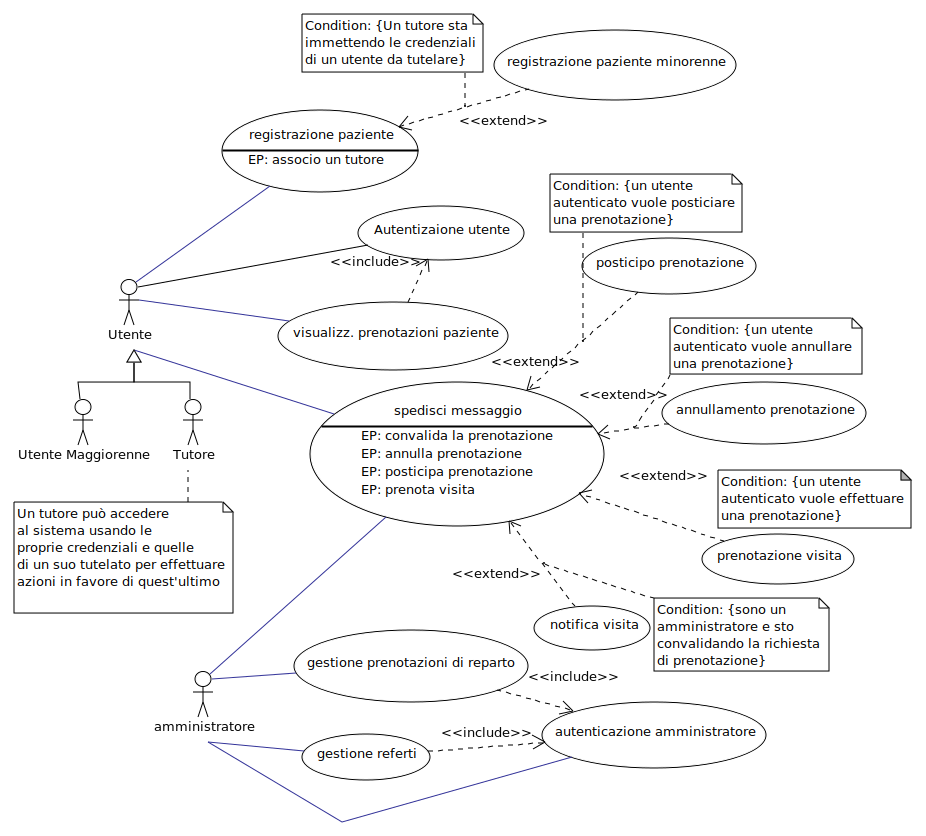
\includegraphics[scale=0.63]{svgs/usecase}
\caption{\textit{Use Case Diagram}.}
\label{fig:ucd}
\end{figure}

\section{Casi d'uso}
\subsection{Diagramma dei Casi d'Uso}
Per il diagramma dei casi d'uso, si fa riferimento alla figura \vref{fig:ucd}.
Questo è il frutto risultante dalla discussione con il cliente effettuata 
precedentemente nella Sottosezione \vref{subsec:cssdc}.


\subsection{Testo dei Casi d'Uso}\label{subsec:usecasetext}
Dopo aver fornito al cliente il diagramma dei Casi d'Uso, e dopo esserci soffermati
sulle richieste dei clienti «\textit{concentrandoci sullo scopo}», abbiamo
ideato alcuni possibili scenari d'interazione con il sistema, allo scopo di
concretizzare maggiormente il problema e  raccogliere le impressioni
del cliente in merito alla soluzione\footnote{R.S. Pressman: ``Principi di Ingegneria del Software''. McGraw-Hill
editore.} in via di
proposizione. In particolare è interessante sapere:
\begin{itemize}
\item In quale modo si caratterizzerebbe un "buon" output generato da una 
	soluzione di successo, o come si arriva, aggiungiamo, ad una soluzione
	di insuccesso?
\item È possibile mostrare o descrivere l'ambiente operativo in cui verrà 
	utilizzata la soluzione?
\end{itemize}
Per raccogliere questi requisiti funzionali, ci siamo interessati ad uno
\textbf{stile concreto} per la scrittura dei casi d'uso\footnote{C. Larman: op. cit.}:
 di fatti ora  «\textit{le decisioni sull'interfaccia utente sono incorporate nel 
 testo del caso d'uso}», per meglio comprendere come l'interazione dell'utente 
 con il sistema possa soddisfare i desideri del committente.

\pagebreak

\begin{description}
\item[Nome del caso d'uso]
       	Accedere al sistema

\item[Attore primario]
        L'utente

\item[Parti interessate e interessi]
        L'utente: vuole accedere nel sistema informativo come sè stesso (Paziente
        maggiorenne) o come il suo tutelato (Paziente minorenne).

\item[Pre-condizioni]
	Nessuna.

\item[Garanzia di successo]
        Il sistema visualizzerà l'interfaccia di default.

\item[Scenario principale di successo]
\begin{enumerate}
\item Il sistema presenta all'utente il meccanismo di autenticazione
\item L'utente inserisce Codice Fiscale e Password del paziente al quale sono
	associate le richieste di servizio.
\item Il sistema verifica la correttezza delle credenziali e le riconosce valide
\item Il sistema consente l'accesso e visualizza l'interfaccia di default.
\end{enumerate}

\item[Estensioni]
\begin{description}
	\item[Estensione A]
	\medskip
	
	\begin{description}
	\item[3]
	Il sistema non riconosce come valide le credenziali del paziente.
	\item[4]
	Il sistema non consente l'accesso visualizzando un messaggio d'errore.
	\item[5]
	Il sistema ritorna al meccanismo di autenticazione.
	\end{description}
	
\end{description}

\begin{description}
	\item[Estensione B]
	\medskip
	
	\begin{description}
	\item[3]
	Il sistema riconosce il paziente come minorenne.
	\item[4]
	Il sistema informa l'Utente che deve fornire le credenziali di Tutore.
	\item[5]
	Il Tutore inserisce le sue credenziali di Codice Fiscale e Password.
	\item[6]
	Il sistema verifica la correttezza delle credenziali e le riconosce valide.
	\item[7] 
	Il sistema consente l'accesso e visualizza l'interfaccia di default.
	\end{description}
	
\end{description}

\begin{description}
	\item[Estensione C]
	\medskip
	\begin{description}
	\item[B]
	\begin{description}
	\item[6]
	Il sistema verifica la correttezza delle credenziali e le riconosce valide.
	\item[7] 
	Il sistema non riconosce come valide le credenziali del paziente.
	\item[8]
	Il sistema non consente l'accesso visualizzando un messaggio d'errore.
	\item[9]
	Il sistema ritorna al meccanismo di autenticazione.
	\end{description}
	\end{description}
	
\end{description}


\item[Requisiti non funzionali]
\begin{itemize}
\diam  Le credenziali dell'Amministratore devono essere cablate all'interno del
	sistema informativo.
\end{itemize}
\end{description}

\begin{center}
\line(1,0){250}
\end{center}

\begin{center}
\line(1,0){250}
\end{center}

\begin{description}
\item[Nome del caso d'uso] Registrare il paziente
\item[Attore primario]
	L'utente (del sistema): il paziente maggiorenne od il tutore del paziente minorenne

\item[Parti interessate ed interessi]
	L'utente: vuole registrare o sé stesso, o il paziente minorenne di cui ha tutela

\item[Pre-condizioni]
	Nessuna

\item[Garanzia di successo]
	Il sistema visualizzerà all'utente un messaggio di avvenuta registrazione

\item[Scenario principale di successo]

\begin{enumerate}
	\item L'utente sceglie l'opzione di registrazione
	\item L'utente inserisce i dati del paziente che dovrà ricevere le cure
	\item L'utente richiede la registrazione
	\item L'utente riceve la notifica di avvenuta registrazione con una notifica tramite il sistema
\end{enumerate}

\item[Estensioni]
\begin{description}
	\item[Estensione A]
	\medskip
	
	\begin{description}
	\item[4] L'utente richiede la registrazione con successo in quanto è un paziente maggiorenne
	\end{description}
\end{description}


\begin{description}
	\item[Estensione B]
	\medskip
	
	\begin{description}
	\item[4] 
	\begin{enumerate}
		\item Il sistema richiede all'utente l'associazione delle credenziali del tutore, in quanto il paziente in fase di registrazione è minorenne
		\item Il tutore inserisce le proprie credenziali
		\item Il sistema conferma la presenza del tutore all'interno del sistema 
		\item Il sistema effettua la registrazione del paziente minorenne e dell'associazione con il tutore utente del sistema
	\end{enumerate}
	\end{description}
\end{description}

\begin{description}
	\item[Estensione C]
	\medskip
	
	\begin{description}
	\item[4] 
	\medskip
	
	Il sistema informa l'utente della mancata registrazione del paziente, specificando quali siano i campi che sono stati ignorati in fase di registrazione
	\end{description}
\end{description}

\begin{description}
	\item[Estensione D]
	\medskip
	
	\begin{description}
	\item[4B (3)] 
	\medskip
	
	\begin{enumerate}
	\item Il sistema informa il tutore che lui stesso non esiste all'interno del sistema
	\item Il tutore annulla la registrazione del minore 
	\end{enumerate}
	\end{description}

\end{description}
\item[Requisiti non funzionali]
\begin{itemize}
\diam Il sistema informativo deve poter prevedere autentificazione per i vari
	utenti e per l'amministratore, ed in più il paziente minorenne può accedere solamente mediante
	la supervisione del tutore; è richiesta autenticazione  sia per il
	paziente minorenne, sia per il tutore.
\end{itemize}
\end{description}
\begin{center}
\line(1,0){250}
\end{center}

\pagebreak

\begin{center}
\line(1,0){250}
\end{center}



\begin{description}
\item[Nome del caso d'uso]
        Contattare l'amministratore

\item[Attore primario]
        L'utente (del sistema)

\item[Parti interessate e interessi]
\begin{itemize}
\diam L'utente: vuole contattare l'amministratore.
\diam L'amministratore: riceve la richiesta dell'utente
\end{itemize}

\item[Pre-condizioni]
        L'utente è già autenticato come un paziente (o come se stesso, o come il 
        paziente di cui è tutore).

\item[Garanzia di successo]
        Il sistema visualizzerà un messaggio di avvenuta ricezione.

\item[Scenario principale di successo]
\begin{enumerate}
\item L'utente visualizza la lista delle prenotazioni.
\item L'utente sceglie l'opzione d'inviare un messaggio all'amministratore del reparto.
\item L'utente richiede il posticipo dell'ultima prenotazione. 
\item L'utente invia la richiesta.
\item L'utente viene informato dal sistema dell'avvenuto invio.
\item L'amministratore riceve la richiesta, che viene valutata.
\item L'amministratore effettua il posticipo della visita interagendo con il sistema.
\item L'utente viene informato dal sistema dell'avvenuta gestione della richiesta.
\item Dopo la visita, L'amministratore assocerà il referto alla prenotazione.
\end{enumerate}

\item[Estensioni]
\begin{description}
	\item[Estensione A]
	\medskip
	
	Inoltre il tutore deve inserire le sue credenziali 
	all'interno del sistema per ogni operazione con il sistema: punti 1 e 5.
	
\end{description}
                
\begin{description}
	\item[Estensione B]
	\medskip
	
	\begin{description}
	\item[4]
	L'utente richiede l'annullamento della prenotazione. 
	\end{description}
\end{description}

\begin{description}
	\item[Estensione C]
	\medskip
	
	\begin{description}
	\item[8]
	L'utente viene informato dal sistema dell'avvenuta gestione della richiesta.
	\item[9]
	L'amministratore riceve la gestione di un caso urgente.
	\item[10]
	L'amministratore sposta la prenotazione dell'utente in questione
	\item[11]
	L'utente riceve la notifica che la sua prenotazione è stata spostata
	\end{description}
\end{description}
\item[Requisiti non funzionali]
\begin{itemize}
\diam Il sistema informativo deve poter prevedere autenticazione per i vari
	utenti e per l'amministratore, ed in più il paziente minorenne può accedere solamente mediante
	la supervisione del tutore; è richiesta autenticazione  sia per il
	paziente minorenne, sia per il tutore.
\end{itemize}
\end{description}



\begin{center}
\line(1,0){250}
\end{center}


\begin{description}
\item[Nome del caso d'uso]
        Effettuare una prenotazione

\item[Attore primario]
        L'utente (del sistema)

\item[Parti interessate e interessi]
\begin{itemize}
\diam L'utente: vuole effettuare una prenotazione.
\diam L'amministratore: riceve la richiesta dell'utente.
\end{itemize}

\item[Pre-condizioni]
        L'utente è già autenticato come un paziente (o come se stesso, o come il 
        paziente di cui è tutore).

\item[Garanzia di successo]
        Il sistema visualizzerà un messaggio di avvenuta assegnazione.

\item[Scenario principale di successo]
\begin{enumerate}
\item L'utente seleziona verso quale reparto inoltrare la sua richiesta.
\item L'utente fornisce una breve descrizione dei sintomi.
\item L'utente inoltra la richiesta verso il sistema.
\item Il sistema visualizza l'elenco delle richieste pendenti all'amministratore.
\item L'amministratore vaglia la richiesta pervenutagli, assegnando una prenotazione
	dipendentemente al grado di priorità.
\item Il sistema memorizza la prenotazione, ed invia una notifica all'utente, ed
	un'altra all'amministratore.
\item L'utente riceve una notifica dal sistema di avvenuta assegnazione della
	prenotazione.
\item L'amministratore riceve la notifica e ritorna all'interfaccia di default.
\end{enumerate}

\item[Estensioni]
\begin{description}
	\item[Estensione A]
	\medskip
	
	\begin{description}
	\item[1]
	Se il paziente in questione è un minorenne, il reparto scelto è per forza 
	quello di pediatria.
	\item[3] Il tutore deve inserire le sue credenziali 
	all'interno del sistema per ogni operazione con il sistema.
	\end{description}
\end{description}
\item[Requisiti non funzionali] 
\begin{itemize}

        \diam L'amministratore deve essere in grado di ``stampare'' su interfaccia grafica.
\diam L'amministratore deve essere in grado di notificare la prenotazione tramite
	un sistema di messaggi interno al sistema.
\diam Il sistema informativo deve poter prevedere autenticazione per i vari
	utenti e per l'amministratore, ed in più il paziente minorenne può accedere solamente mediante
	la supervisione del tutore; è richiesta autenticazione  sia per il
	paziente minorenne, sia per il tutore.
\diam L'amministratore deve poter visualizzare un calendario settimanale ove
	poter convalidare la prenotazione delle visite, e visualizzare gli slot
	orari già occupati.
\end{itemize}       
\end{description}


\begin{center}
\line(1,0){250}
\end{center}

\pagebreak

\begin{center}
\line(1,0){250}
\end{center}


\begin{description}
\item[Nome del caso d'uso]
        Visualizzare lo storico delle prenotazioni

\item[Attore primario]
        L'utente (del sistema)

\item[Parti interessate e interessi]
        L'utente: vuole accedere alle informazioni delle prenotazioni

\item[Pre-condizioni]
        L'utente è già autenticato come un paziente (o come se stesso, o come il 
        paziente di cui è tutore), e deve avere prenotazioni a lui associate
        all'interno del sistema.

\item[Garanzia di successo]
        Il sistema visualizzerà le prenotazioni.

\item[Scenario principale di successo]
\begin{enumerate}
\item L'utente visualizza la lista delle prenotazioni.
\item L'utente seleziona una particolare prenotazione.
\item L'utente sceglie di visualizzare il referto associato alla prenotazione.
\item Il sistema visualizza il referto a video
\end{enumerate}

\item[Estensioni]


\begin{description}
	\item[Estensione A]
	\medskip
	\begin{description}
	\item[3]
	Il paziente non trova alcun referto da visualizzare: si interrompe lo
	scenario
	\end{description}
	
\end{description}

\begin{description}
	\item[Estensione B]
	\medskip
	
	Inoltre il tutore deve inserire le sue credenziali 
	all'interno del sistema per ogni operazione con il sistema: punti 1 e 3.
	
\end{description}

\begin{description}
	\item[Estensione C]
	\medskip
	
	\begin{description}
	\item[4]
	L'utente del sistema, può richiedere di salvare il referto come file
	all'interno del suo sistema.
	\end{description}
	
\end{description}



\item[Requisiti non funzionali]
        \begin{itemize}
        \diam L'amministratore deve essere in grado di ``stampare'' su interfaccia grafica.
\diam L'utente deve essere in grado di ``stampare'' su file.
\diam L'amministratore deve essere in grado di inserire i referti nel sistema
	tramite inserimento di testo.
        \end{itemize}
\end{description}

\begin{center}
\line(1,0){250}
\end{center}


\begin{description}
\item[Nome del caso d'uso]
       	Accedere al sistema

\item[Attore primario]
        L'amministratore

\item[Parti interessate e interessi]
        L'amministratore: vuole accedere nel sistema informativo.

\item[Pre-condizioni]
	Nessuna.

\item[Garanzia di successo]
        Il sistema visualizzerà l'interfaccia di default, ovvero il calendario
        delle prenotazioni.

\item[Scenario principale di successo]
\begin{enumerate}
\item Il sistema presenta all'amministratore il meccanismo di autenticazione
\item L'amministratore inserisce Nome Utente e Password
\item Il sistema verifica la correttezza delle credenziali e le riconosce valide
\item Il sistema consente l'accesso e visualizza l'interfaccia di default, ovvero .
	il calendario delle prenotazioni.
\end{enumerate}

\item[Estensioni]
\begin{description}
	\item[Estensione A]
	\medskip
	
	\begin{description}
	\item[3]
	Il sistema non riconosce come valide le credenziali dell'amministratore.
	\item[4]
	Il sistema non consente l'accesso visualizzando un messaggio d'errore.
	\item[5]
	Il sistema ritorna al meccanismo di autenticazione.
	\end{description}
	
\end{description}


\item[Requisiti non funzionali]
\begin{itemize}
\diam  Le credenziali dell'Amministratore devono essere cablate all'interno del
	sistema informativo.
\end{itemize}
\end{description}

\begin{center}
\line(1,0){250}
\end{center}




\begin{description}
\item[Nome del caso d'uso]
       	Inserire i referti dei pazienti

\item[Attore primario]
        L'amministratore

\item[Parti interessate e interessi]
        L'amministratore: inserisce il referto all'interno delle prenotazioni alla fine
        di associarlo alla prenotazione, e quindi alla visita precedentemente 
        assegnata.

\item[Pre-condizioni]
	L'amministratore si autentica ed accede nel sistema.
        Deve essere presente all'interno del sistema una prenotazione del paziente,
        e la visita associata alla prenotazione deve essere avvenuta.

\item[Garanzia di successo]
        Il sistema visualizzerà l'associazione tra prenotazione ed il referto.

\item[Scenario principale di successo]
\begin{enumerate}
\item L'amministratore richiede di poter visualizzare le prenotazioni.
\item L'amministratore seleziona una particolare prenotazione.
\item L'amministratore seleziona l'opzione ``Inserisci referto''
\item L'amministratore inserisce i dati del referto in modalità testuale.
\item Il sistema associa il referto alla visita medica
\item Il sistema visualizza l'associazione tra la prenotazione ed il referto medico.

\end{enumerate}

\item[Estensioni]
	Nessuna


\item[Requisiti non funzionali]
\begin{itemize}
\diam L'amministratore deve essere in grado di inserire i referti nel sistema
	tramite inserimento di testo.
\end{itemize}
\end{description}

\begin{center}
\line(1,0){250}
\end{center}


\begin{description}
\item[Nome del caso d'uso]
       	Modificare i referti dei pazienti

\item[Attore primario]
        L'amministratore

\item[Parti interessate e interessi]
        L'amministratore: vuole modificare un referto medico.

\item[Pre-condizioni]
	L'amministratore è già autenticato con successo.

\item[Garanzia di successo]
        Il sistema visualizzerà l'associazione tra prenotazione ed il nuovo 
        referto.

\item[Scenario principale di successo]
\begin{enumerate}
\item L'amministratore sceglie l'opzione ``Modifica referto''.
\item Il sistema visualizza l'interfaccia per la modifica dei reperti medici.
\item L'amministratore inserisce i dati modificati del referto.
\item L'amministratore salva il nuovo referto.

\end{enumerate}

\item[Estensioni]
	Nessuna


\item[Requisiti non funzionali]
\begin{itemize}
\diam L'amministratore ``stampa'' su interfaccia grafica.
\end{itemize}
\end{description}



\begin{center}
\line(1,0){250}
\end{center}


\begin{center}
\line(1,0){250}
\end{center}



\begin{description} 
\item[Nome del Caso d'Uso]
	Gestire le prenotazioni

\item[Attore primario]
        L'amministratore

\item[Parti interessate e interessi]
\begin{itemize}
\diam L'amministratore: vuole visualizzare le richieste di prenotazione 
        e convalidarle.
\diam L'utente: riceve la notifica dell'amministratore.
\end{itemize}


\item[Pre-condizioni]
	L'amministratore si autentica ed accede nel sistema.

\item[Garanzia di successo]
        Il sistema visualizzerà un messaggio di effettuata gestione.

\item[Scenario principale di successo]
\begin{enumerate}
\item L'amministratore visualizza la lista delle prenotazioni pendenti.
\item L'amministratore attribuisce alla prenotazione data priorità e medico. 
\item L'amministratore conferma la prenotazione.
\item L'utente riceve dal sistema la notifica di conferma della prenotazione.
\end{enumerate}

\item[Estensioni]
\begin{description}
	\item[Estensione A] (scenario di modifica delle prenotazioni)
	\medskip
	
	\begin{description}
	\item[3]
	\begin{enumerate}
	\item L'amministratore sceglie la prenotazione da posticipare
	\item Il sistema visualizza l'interfaccia di modifica della prenotazione,
		mostrando le altre date libere all'interno del calendario.
	\item L'amministratore posticipa all'interno di uno slot orario libero
		una prenotazione già precedentemente convalidata.
	\item L'amministratore notifica al paziente la cui prenotazione è stata
		posticipata.
	\item L'amministratore conferma la nuova prenotazione, in sostituzione di 
		quella modificata.
	\end{enumerate}
	\end{description}
	
\end{description}
                

\item[Requisiti non funzionali]
\begin{itemize}
\diam Il sistema informativo deve poter prevedere autenticazione per i vari
	utenti e per l'amministratore.
\end{itemize}
\end{description}



\begin{center}
\line(1,0){250}
\end{center}


\section{Glossario}\label{sec:glossario}
Si produce il glossario visionabile in Tabella \vref{tab:gloss}. 

\begin{table}[!t]
\begin{tabularx}{\columnwidth}{lX}
\toprule
Nome & Definizione\\
\midrule
\textbf{Paziente} & È un utilizzatore del sistema, dal quale otterrà valore tramite 
	l'effettuazione di una visita.\\
\textbf{Paziente minorenne} & Il paziente minorenne è un \textsc{Paziente} che, per 
	usufruire dei servizi del sistema, ha  bisogno di:
	fornire le proprie credenziali ( unicamente all'atto dell'autenticazione),
	essere associato ad uno ed un solo tutore, e
	fornirne le credenziali del tutore.
 	\\
\textbf{Paziente maggiorenne} & Il paziente maggiorenne è un utilizzatore del sistema 
	che, per usufruire dei servizi del sistema, ha bisogno unicamente di
	fornire le proprie credenziali ( unicamente all'atto dell'autenticazione).
	Assieme al Tutore è un \textbf{Utente} del sistema.\\
\textbf{Tutore} & Il tutore è un utilizzatore del sistema che può accedere a questo
	usando le sue credenziali e quelle del suo tutelato, allo scopo di
	garantire a quest'ultimo i servizi offerti al sistema. Assieme al Paziente
	maggiorenne è un \textbf{Utente} del sistema.\\
\textbf{Amministratore} & L'amministratore è unico, per reparto, e preesistente nel 
	sistema. Egli si occupa di classificare le richieste dei pazienti ed 
	assegnare loro una prenotazione, di cambiare una prenotazione preesistente 
	qualora vi sia l'esigenza, da lui considerata, di privilegiarne una
	a priorità maggiore (nei confronti di altre già concordate).\\
\textbf{Prenotazione} & Una prenotazione è un oggetto creato dall'amministratore e 
	riferito ad un unico paziente che indica la data, la sala dalla quale
	segue l'indicazione di un reparto, per cui il dato paziente ha richiesto 
	una visita. Un insieme di prenotazioni è detto \textbf{storico}\\
\textbf{Reparto} & Il reparto è il luogo dove avvengono le diverse tipologie di visite
	in base alla distinzione tra Ortopedia e Pediatria. Ogni reparto è dotato
	di 2 sale (distinte).\\
\textbf{Sala} & La sala è il luogo dove può avvenire, in ogni ora prefissata, una
	sola visita\\
\textbf{Referto} & Il referto è un oggetto rilasciato al paziente al termine della
	visita. Ogni visita produce uno ed un solo referto, il quale è associato 
	ad un unico paziente e può essere controllato da quest'ultimo attraverso 
	il sistema informativo.\\
\textbf{Messaggio} & Un messaggio è formato da 3 parametri: un campo destinatario,
un campo mittente e contenuto del messaggio.
Se il campo destinatario è un paziente allora il mittente sarà un amministratore, 
viceversa, mittente paziente destinatario amministratore.
Può essere una richiesta di visita od una conferma di prenotazione, o una richiesta
di cancellazione o di spostamento della stessa.
\end{tabularx}
\caption{\textit{Glossario}.}
\label{tab:gloss}
\end{table}

